% =====================================================================
%  Prabhavit Gupta, one-page CV template (Allitude - GenAI Engineer)
%  Compile:  tectonic main_Allitude_GenAIEngineer.tex
%  Needs:    photo.jpg in the same folder as this .tex
%  Rules:    ONE PAGE. No em-dashes. Plain voice. Clickable companies.
%            No "sample of my code" line. Salary blank or "negotiable".
%            Never write "no-code" or "Bubble", say "off a legacy stack".
% =====================================================================
\documentclass[a4paper,10pt]{article}

\usepackage[T1]{fontenc}
\usepackage[utf8]{inputenc}
\usepackage[top=0.75cm,bottom=0.75cm,left=1.0cm,right=1.0cm]{geometry}
\usepackage{titlesec}
\usepackage{enumitem}
\usepackage{hyperref}
\usepackage{xcolor}
\usepackage{graphicx}

\definecolor{accent}{HTML}{1F4E78}
\hypersetup{colorlinks=true, urlcolor=accent, linkcolor=accent}
\pagestyle{empty}
\setlength{\parindent}{0pt}

\titleformat{\section}{\large\bfseries\color{accent}}{}{0em}{}[\vspace{-0.6em}\rule{\textwidth}{0.8pt}]
\titlespacing{\section}{0pt}{2pt}{1pt}

\newcommand{\role}[4]{%
 \textbf{#1} \hfill \textbf{#2}\\[1pt]%
 \textit{#3} \hfill \textit{#4}\\[2pt]%
}
\setlist[itemize]{leftmargin=1.2em, itemsep=0pt, topsep=1pt, parsep=0pt}

\begin{document}

% ================= HEADER =================
\begin{minipage}[c]{0.80\textwidth}
 {\Huge\bfseries Prabhavit Gupta}\\[3pt]
 {\color{accent}\large GenAI Engineer, LLM Agents \& Production Systems}\\[6pt]
 {\footnotesize +39 351 610 7807 ~$\vert$~
 \href{mailto:prabhavitg@gmail.com}{prabhavitg@gmail.com} ~$\vert$~
 \href{https://www.linkedin.com/in/prabhavit/}{linkedin.com/in/prabhavit} ~$\vert$~
 \href{https://github.com/prab-gupta}{github.com/prab-gupta} ~$\vert$~
 Venice, Italy}
\end{minipage}\hfill
\begin{minipage}[c]{0.18\textwidth}
 \raggedleft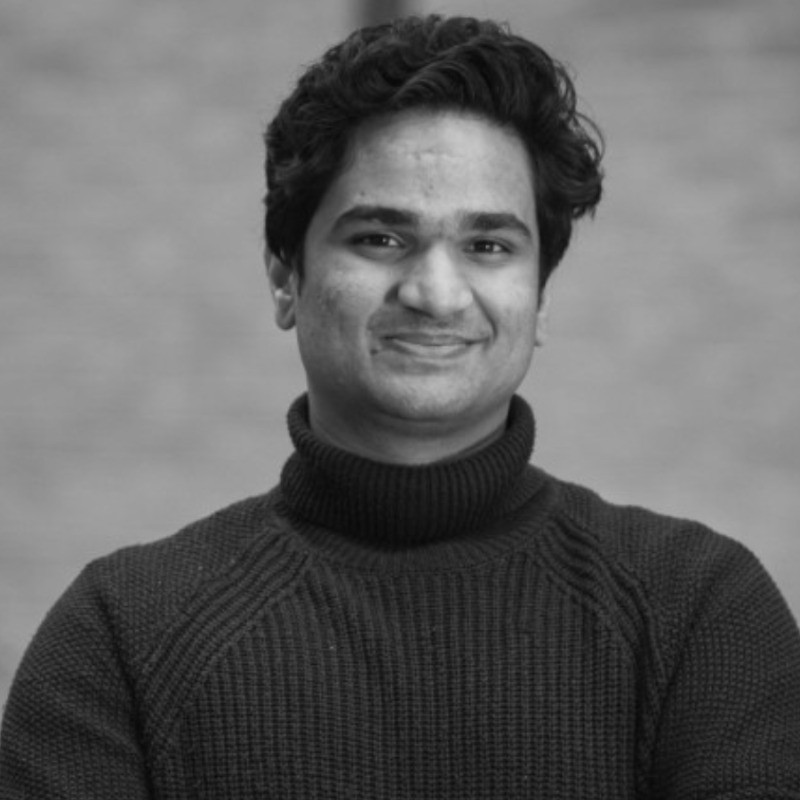
\includegraphics[width=2.0cm]{photo.jpg}
\end{minipage}
\vspace{-2pt}

% ================= SUMMARY =================
\section{Summary}
Full-stack and AI engineer specializing in Generative AI solutions, agentic architectures, and automated knowledge retrieval. Shipped production systems connecting foundational LLMs (Claude, OpenAI) to enterprise APIs, relational databases, and multi-format data pipelines. At FlowSpace, engineered an automated document ingestion agent with human-in-the-loop validation (900+ listings drafted), deployed live customer-facing support agents with confidence-based escalation, and led the platform migration off a legacy stack to Next.js and Laravel (scaling to 4,500+ users). Daily stack: Python, TypeScript, n8n, RAG patterns, and Claude Code.

% ================= SKILLS =================
\section{Skills}
\begin{itemize}
 \item \textbf{Generative AI \& Agentic Systems:} LLM integration (Claude, OpenAI APIs), agentic workflows, RAG architectures, prompt engineering, document automation, semantic knowledge retrieval, human-in-the-loop review, Claude Code, n8n, Eden AI
 \item \textbf{Software Development \& Backend:} Python (FastAPI, data parsing), TypeScript, JavaScript, Node.js, Next.js, Laravel (PHP), REST APIs, OpenAPI, webhooks, asynchronous pipelines, PostgreSQL, Supabase
 \item \textbf{Enterprise Integration \& Delivery:} Rapid prototyping (POC to production), third-party API integrations (OfficeRnD, Nexudus, Google APIs, CRM), schema validation, error handling, Docker, CI/CD, Git/GitHub
 \item \textbf{Testing, QA \& Reliability:} Playwright, unit testing, automated contract testing, logging and observability, Postman, Jira, Figma
\end{itemize}

% ================= EXPERIENCE =================
\section{Experience}

\role{\href{https://flowspace.co}{FlowSpace.co}}{Mar 2024 -- Aug 2026}{Lead Developer \& AI Engineer (Full-time, Freelance)}{London, UK (remote)}
\begin{itemize}
 \item Designed and shipped an automated document ingestion pipeline (TypeScript, Claude, n8n) extracting structured data from multi-format brochures (PDF, web, spreadsheet) with human-in-the-loop review; 900+ listings drafted.
 \item Deployed conversational AI support agents querying live platform records, with confidence scoring and automated fallback to human operators.
 \item Led the core platform migration off a legacy stack to coded Next.js and Laravel, scaling active users from 2,000 to 4,500+.
 \item Integrated OfficeRnD and Nexudus APIs for automated booking synchronization, webhook handling, and data consistency.
 \item Engineered CRM and GTM automations for lead capture, enrichment, intelligent routing, and outbound messaging.
\end{itemize}

\role{\href{https://get2germany.com}{Get2Germany.com}}{Jan 2024 -- May 2024}{Developer \& Automation Specialist (Part-time)}{Berlin, Germany}
Integrated Google APIs and built AI tools in n8n for automated search, knowledge retrieval, and data aggregation, optimizing backend databases.\\[1pt]

\role{\href{https://clubee.com}{Clubee.com}}{Sep 2023 -- Aug 2024}{Developer \& QA (Full-time, Freelance)}{Foetz, Luxembourg}
Integrated enterprise REST APIs across the frontend, ran unit testing and QA, and built shop and federation-dashboard tools.\\[1pt]

\role{\href{https://tractionboard.co}{Tractionboard.co}}{Aug 2023 -- Oct 2023}{Developer (Internship)}{Utrecht, Netherlands}
Integrated OpenAI/ChatGPT APIs and Sendgrid, designed responsive frontend interfaces, and debugged production features.

% ================= FREELANCE PROJECTS =================
\section{Freelance Projects}
\begin{itemize}
 \item \textbf{\href{https://smarturlink.com/}{Urlink}} (2025), Project Manager \& AI-Assisted Developer. Built platform logic and automations using AI-assisted engineering (Claude Code, bolt.new) with Next.js and Supabase.
 \item \textbf{\href{https://ultrastrategy.com}{UltraStrategy}} (2024 to 2025), AI Automation Developer. Built an LLM document extraction tool with n8n and Eden AI for multi-profile data structuring.
 \item \textbf{\href{https://www.qomodo.me/}{Qomodo}} (2024 to 2025), AI Developer. Developed an administrative dashboard for multi-branch enterprise management, implementing Figma designs.
\end{itemize}

% ================= CERTIFICATIONS =================
\section{Certifications}
Microsoft Copilot Studio Agent Academy \textbullet\ Microsoft: Introduction to building AI agents \textbullet\ Microsoft Power Automate \textbullet\ Tray.AI Build Practitioner (Sep 2024)

% ================= EDUCATION =================
\section{Education}
\textbf{Ca' Foscari University of Venice} \hfill Oct 2020 -- Jun 2024\\
BA Philosophy, International Studies \& Economics (Minor: Entrepreneurship)

% ================= AUTH =================
\vspace{2pt}
{\small \textbf{Work authorization:} Italian EU Long Term Residence Permit (no visa sponsorship needed); available immediately. \quad \textbf{Languages:} Hindi (native), English (professional C2), Italian (conversational).}

\end{document}
